\subsubsection{Relations}
Relations describe constraints among events. There are 4 basic relations, explained in the following section. \\

\textbf{Condition - yellow arrow:} This relation states that to execute the event \textbf{B}, event \textbf{A} must be executed or excluded first. See Figure \ref{fig:ConditionRelation}.

\begin{figure}[h!]
\centering
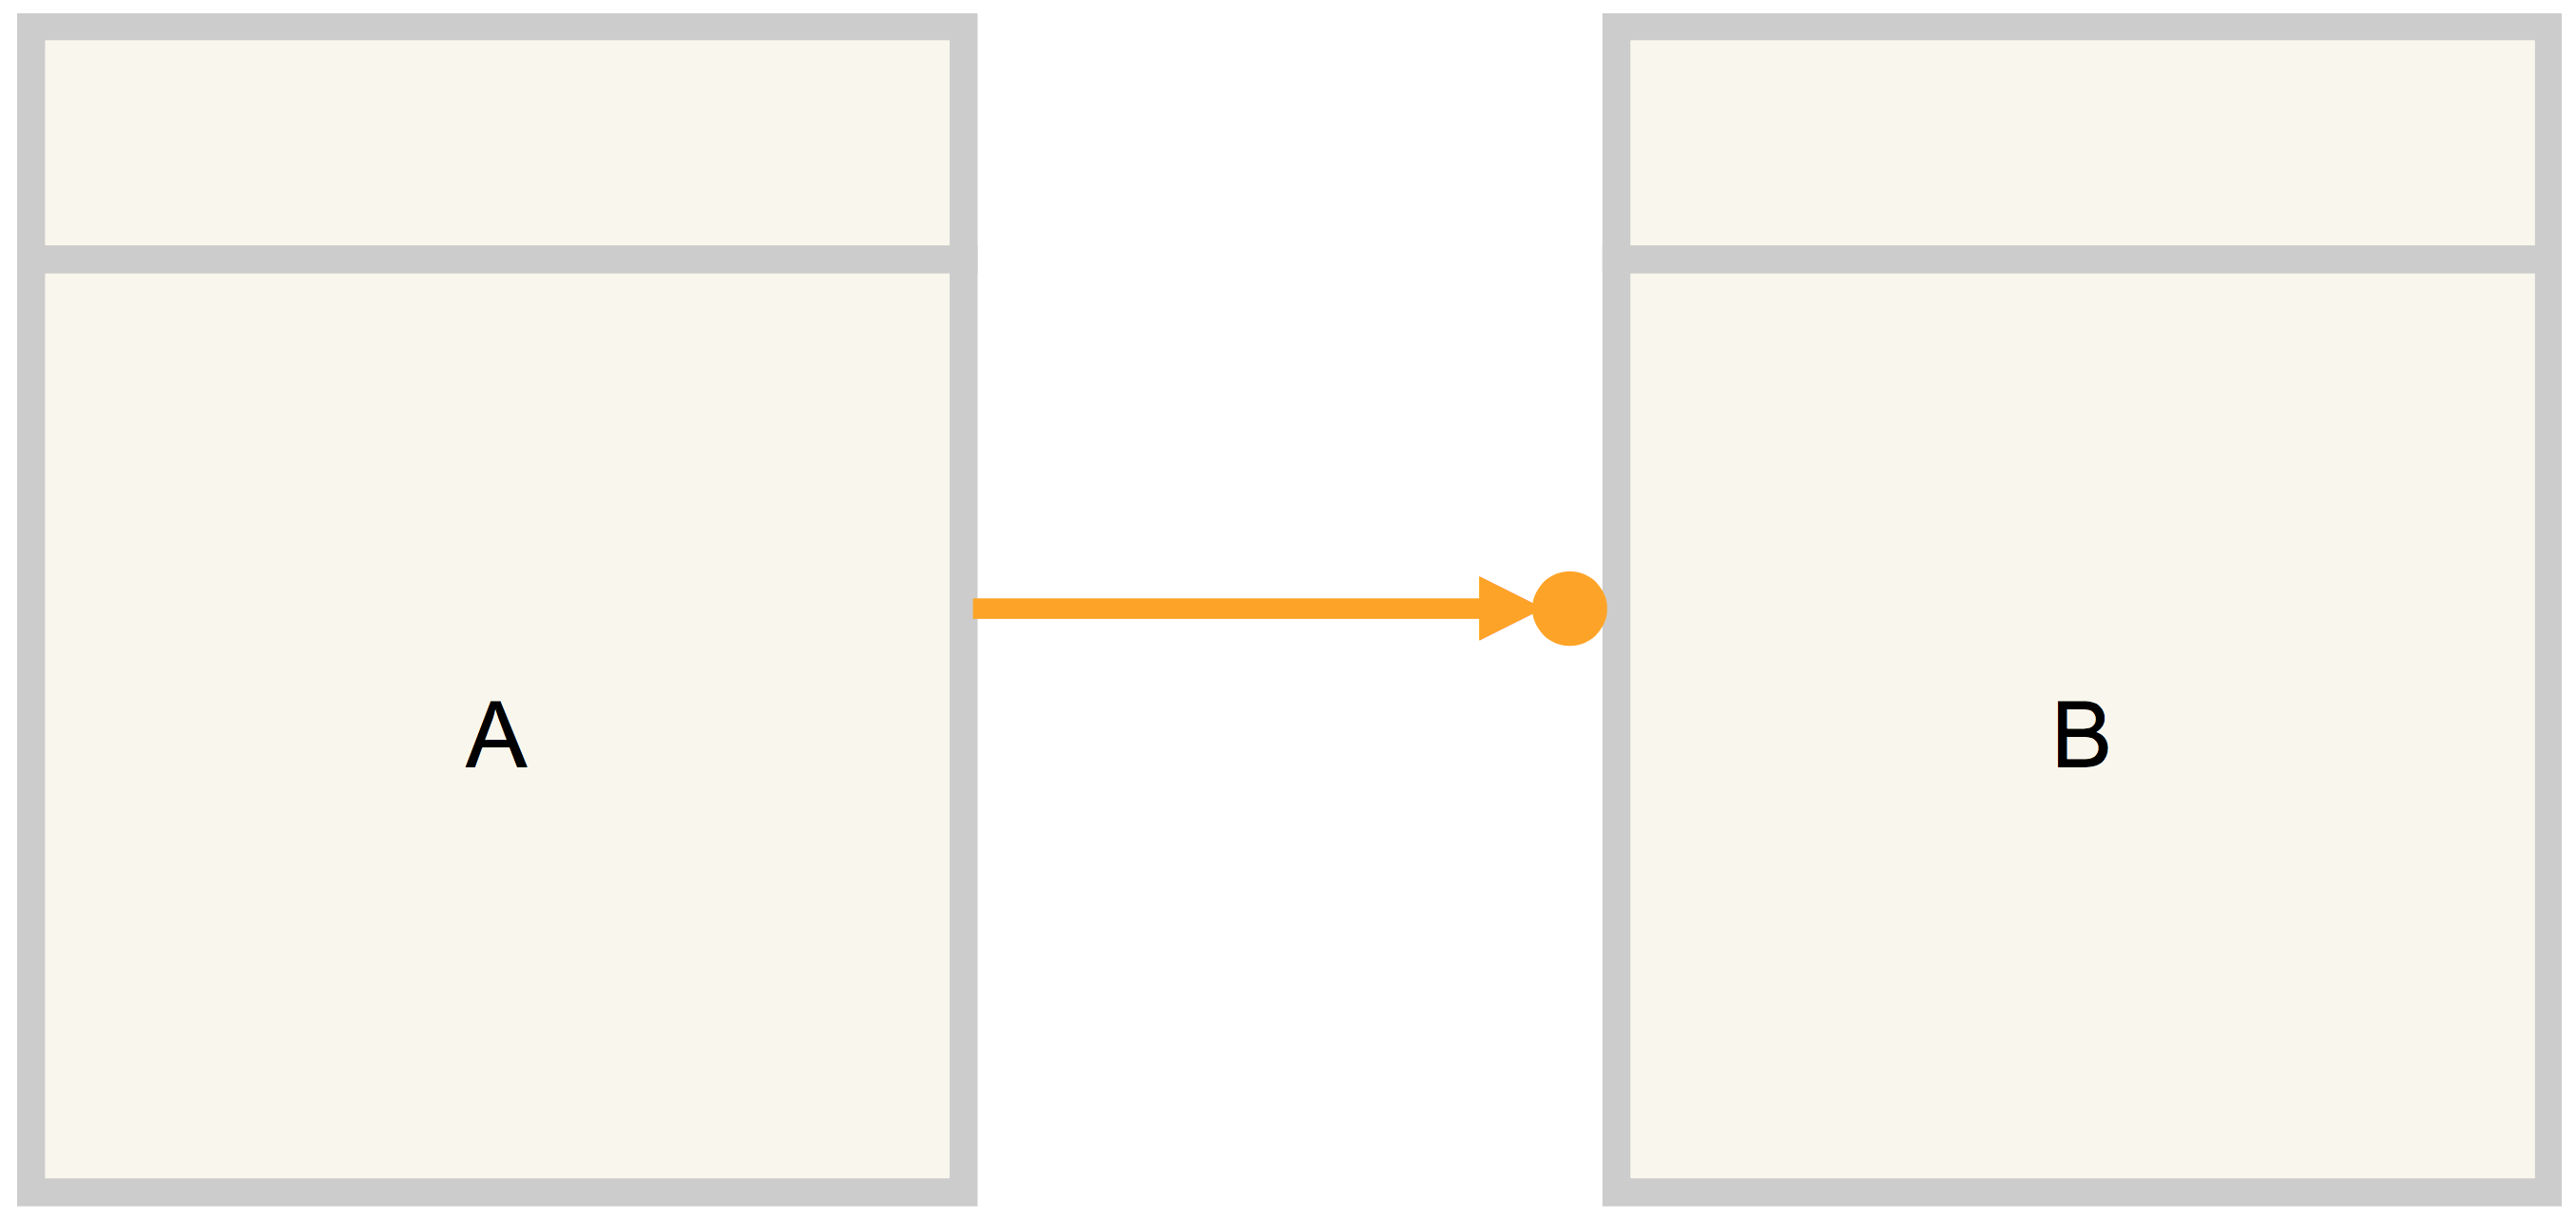
\includegraphics[width=0.5\linewidth]{Figures/conditions}
\caption{\label{fig:ConditionRelation} Illustration of Condition relation between event \textbf{A} and event \textbf{B}}
\end{figure} 

\textbf{Exclude - red arrow:} An exclusion relation states that once event \textbf{A} has been executed, the \textit{Included} boolean of event \textbf{B} must be set to false, such that event \textbf{B} is excluded. Note that an event may exclude itself, meaning once the event has executed, the \textit{Included} value of the event must be set to false such that it is excluded.  See figure \ref{fig:ExclusionRelation}.

\begin{figure}[h!]
\centering
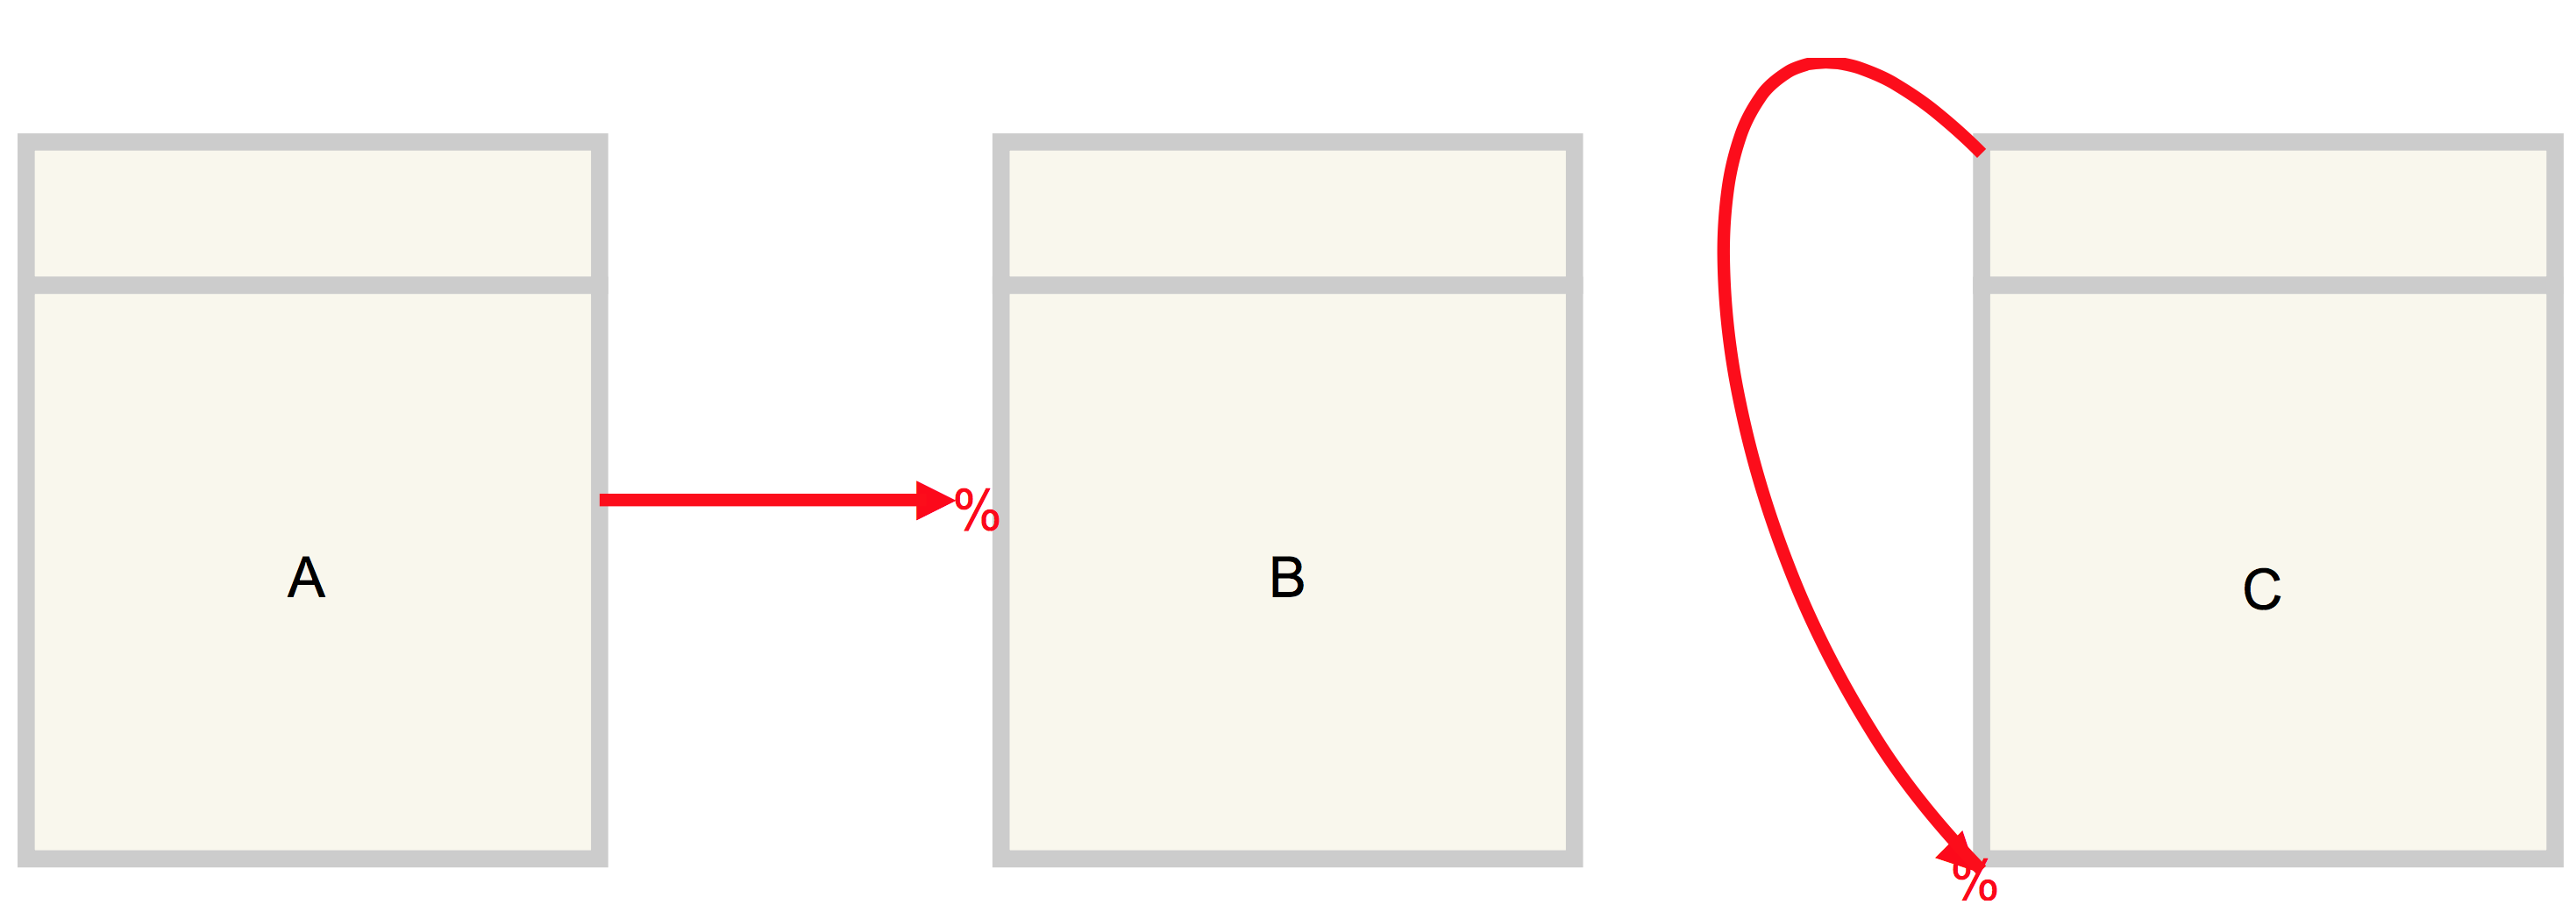
\includegraphics[width=0.8\linewidth]{Figures/exclusion}
\caption{\label{fig:ExclusionRelation} Illustration of exclusion relation between event \textbf{A} and event \textbf{B}. Event \textbf{C} is self excluding.}
\end{figure} 


\textbf{Include - green arrow:} This relation states that event \textbf{A} includes event \textbf{B}. This means that  after the execution of event \textbf{A}, the \textit{Included} value of event \textbf{B} must be set to true, such that event \textbf{B} is included. See Figure \ref{fig:InclusionRelation}

\begin{figure}[h!]
\centering
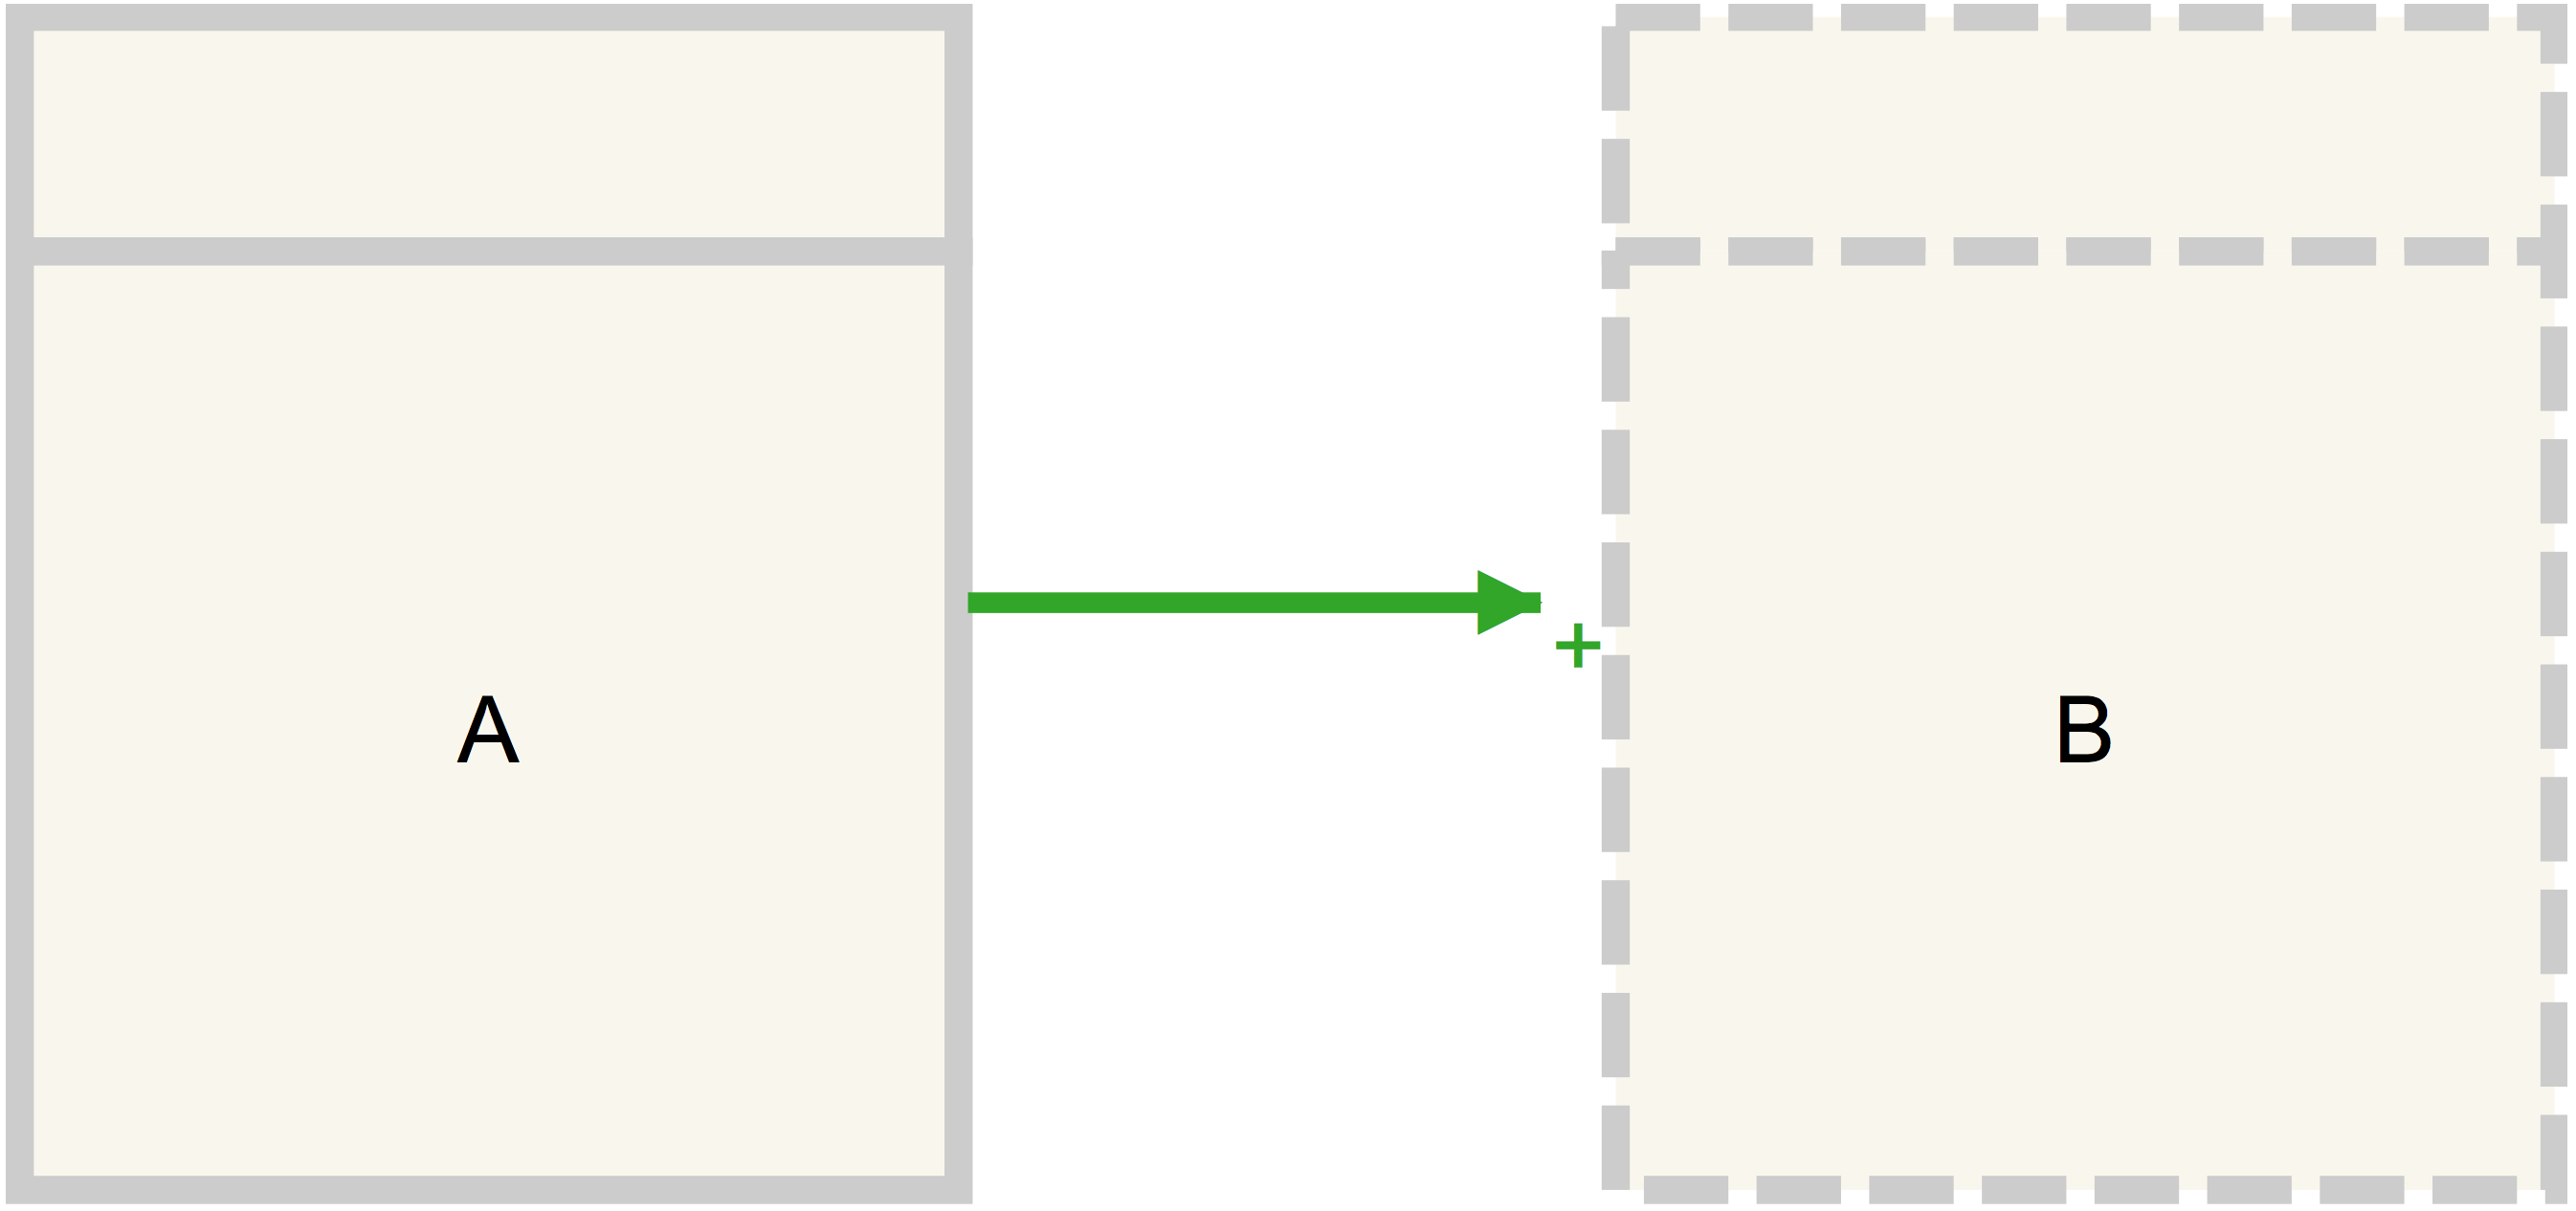
\includegraphics[width=0.5\linewidth]{Figures/inclusion}
\caption{\label{fig:InclusionRelation} Illustration of inclusion relation between event \textbf{A} and event \textbf{B}}
\end{figure} 


\textbf{Response - blue arrow:} The response relation states that once event \textbf{A} is executed, event \textbf{B} is expected to be executed eventually. Once event \textbf{A} has been executed, the \textit{Pending} value of event \textbf{B} must be set to true. See Figure \ref{fig:ResponseRelation}

\begin{figure}[h!]
\centering
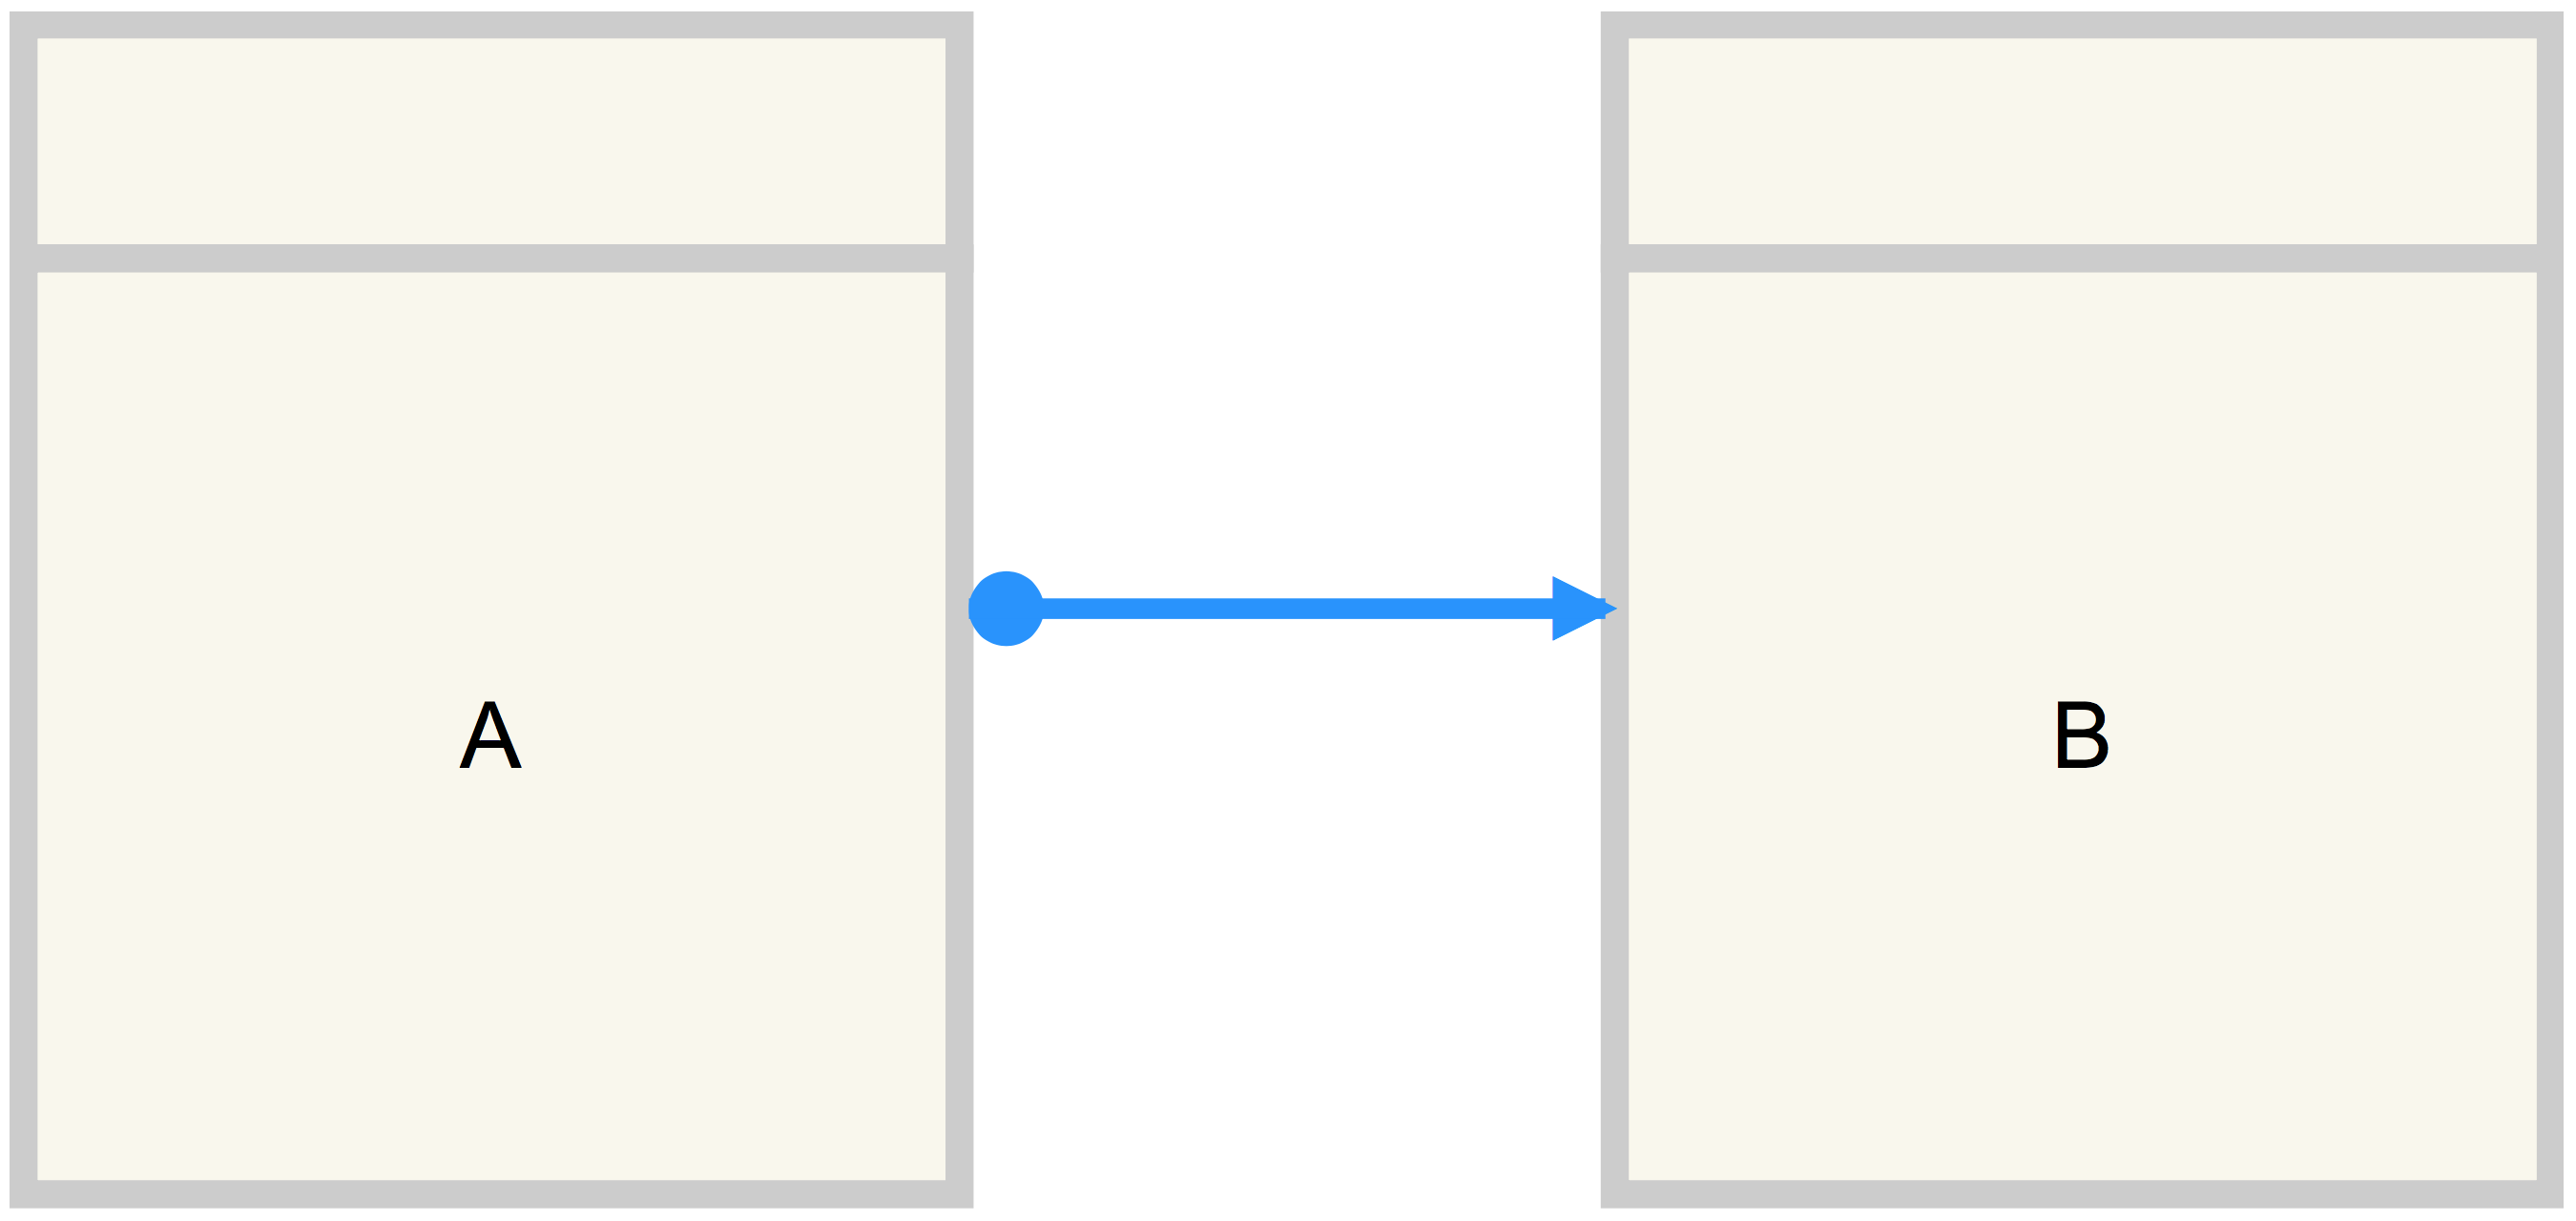
\includegraphics[width=0.5\linewidth]{Figures/response}
\caption{\label{fig:ResponseRelation} Illustration of response relation between event \textbf{A} and event \textbf{B}}
\end{figure} 

To sum up: for an event to be executable, the \textit{Included} value must be true, and each of its condition relations must be either excluded or executed. \\

Furthermore an execution of an event leads to its \textit{Executed} and \textit{Pending} values to be set to true and false respectively. Each of the executed events’ response relations must have their \textit{Pending} value set to true, each of its inclusion relations must have their \textit{Included} value set to true, and its exclusion relations must have their \textit{Included} value set to false. \\

The three concepts: state, events, and relations, will be mirrored in the system.